% !TeX spellcheck = en_US

\chapter{Groundwork}
This chapter covers the basic technologies and terms used throughout the following chapters.



\section{MARS Websuite}
The MARS Websuite is the web application of the MARS working group. It allows the user to prepare and start simulation runs from within the web browser.\\
The original Websuite has a monolithic structure, meaning it is a traditional, single application with many responsibilities, parts and technologies. The new Websuite contains of over 20 independent micro-services.\\
This work focuses on extracting the front-end of the fullstack application into a single micro-service. While doing so, the inherited components are to be reevaluated, redesigned and if needed, rewritten.


\subsection{Data Types}
\label{sec:data-types}
The Websuite supports several data types, which are used to initial the layers inside the actual simulation.

\subsubsection{Table-based}
This import type supports CSV-files with table data that refers to a specific GPS location. An Example would be the starting positions of agents in a model.

\subsubsection{Time-series}
The time-series import supports CSV-files with data that changes over time. An example is data, containing average temperatures per day over the duration of the desired simulation time.

\subsubsection{Geographic-Information-System (GIS)}
Data with a geographical representation can be imported with the GIS import. It supports the most common file types for GEO-processing, which are:
\begin{itemize}
	\item AciiGrid (*.asc)
	\item GeoTIFF (*.tif)
	\item GeoJSON (*.json)
	\item Shapefile (*.shp, *.shx, *.dbf and additional optional files)
\end{itemize}

\subsubsection{Grid-potential-field}
This data type allows the usage of potential-fields, which contains a grid of percentage values. These grids allow the calculation of distances to non moving objects prior to the simulation and hereby reduce simulation time. The file-ending is \textit{.csv}

\subsubsection{Geo-potential-field}
Geo-potential-field is a specialized grid-potential-field that allows the use of GPS coordinates. The file-ending is \textit{.csv}.

\subsubsection{Obstacle}
Obstacle-layer is a gird that contains obstacles. This can be used to limit agent movement. The file-ending is \textit{.csv}.



\section{Micro-services}
\label{sec:micro-services}
Micro-services describes a software architecture, where the software is split up into small, independent components. These components are loosely coupled and communicate over the network. Each so called service runs in its own process and potentially on a different machine.


\subsection{History}
The concept of handling growing complexity in software is not a new one. The first known thoughts about software structure go back to \citeauthor{conway1968committees}'s law \citeyearpar{conway1968committees}. He claims that organizations tend to structure software systems in a way that matches its hierarchy.\\
A more recent approach towards handling complexity is Service-Oriented Architecture (SOA) by \cite{as2005service}. SOA is described as an architecture, were independent services communicate with each other over the network.\\
The term micro-services was introduced by \cite{martinfowler2014microservices}. Their approach is a more specific version of SOA. This is why micro-services are often referred to as \enquote{SOA done right}.\\
Virtual machines allow the virtualization a whole operating system with its hardware. Containerization software like docker, makes it possible to virtualize on a process level. This significantly reduces overhead and allows independent deployments, as a result the popularity of micro-services has strongly increased over the past 2 years.


\subsection{Single responsibility}
Big, monolithic application grow in size and complexity during their existence. This results into higher costs for maintenance and enhancements. Microservices reduce complexity by splitting the application into smaller logical parts.\\
The definition of how small a service has to be varies, \cite{newman2015building} e.g. claims that micro-services should follow the \enquote{Single responsibility} principle by \cite{martin2003agile}. This states that a given component should have only one reason to change, which results in each component having only one responsibility.


\subsection{Autonomy}
Micro-services are loosely coupled, which means that they can be developed and deployed separately. Each service runs in its own process and communicates with other services over the network layer. It is therefore possible to scale up single services, without having to scale the whole application.



\section{AngularJS}
\label{sec:angularjs}
The WebUI front-end is written with the JavaScript framework AngularJS v1.5. Angular was created by Miško Hevery at Brat Tech LLC in the year 2010 and is under active development by Google Inc. \\
The framework extends HTML5 and JavaScript by various paradigms and patterns, in order to make the development of single-page web applications more appealing. The most relevant features are the \textit{Templating Engine}, \textit{Two Way Data-Binding}, \textit{Model–view–viewmodel} and \textit{Dependency Injection}.


\subsection{Template Engine}
The Angular template is the HTML code, written by the developer. Angular combines this HTML with the model data to render a dynamic view. It has the following features.

\subsubsection{Directives}
Directives are Angular's method of extending HTML by new elements with JavaScript logic attached. This can be used to create reusable, parameterized components.

\subsubsection{Markup}
The templating engine allows the user to reference models from the controller to enrich the HTML with model data. This i done with the double curly brackets notation.

\subsubsection{Filter}
Filters allow formating of input data inside the HTML. Angular has build-in filters for common tasks like formating \textit{numbers} \textit{currencies} or \textit{dates} as well as converters to \textit{uppercase} or \textit{lowercase}. It is also possible to create custom filters based on individual needs.

\subsubsection{Form controls}
The use of form controls allows the validation of form-data in real time. Form elements can be validated against certain gates to detect false user input before it is sent to the back-end.\\
This is possible, because every form field has a JavaScript class that holds validation data. Also CSS error classes exist, which allow to easily visualize false inputs.


\subsection{Model–view–viewModel (MVVM)}
Angular takes advantage of the \textit{Model View Controller} (MVC) pattern, which separates the model that holds the data, the view that is displayed to the user and the controller that holds the logic.\\
Angular's implementation is closer to an Model–view–viewModel (MVVM) approach, because it uses a viewModel inside the controller component. Besides containing the controller logic, the viewModel also holds functions for converting data, which keeps the view clean of logic.

\subsubsection{Model}
The Model  is responsible for storing the current state of the application.

\subsubsection{View}
The View is the HTML, that exists, once Angular has interpreted the template and the appertaining data.

\subsubsection{ViewModel}
\label{sec:viewModel}
The viewModel manages data consistency between the model and view. The Controller sets the initial state of the ViewModel and adds values and functions to it. This added functionality defines the behavior of the application. Inside the view, data can also be read and altered. This data is propagated back to the model.


\subsection{Two Way Data-Binding}
\label{sec:tw-binding}
Angular's two way data-binding is responsible for the communication of MVVM components. The data is bound to a Model, which always holds the most recent state of the application. Changes to the data are always passed to the model and read from it. This means that the controller and the view always operate on the same state. This process is visualized in figure \ref{fig:tw-databinding}.\\
The need to write boilerplate code, for transferring states between the HTML view and the JavaScript controller is hereby removed.

\begin{figure}[H]
	\centering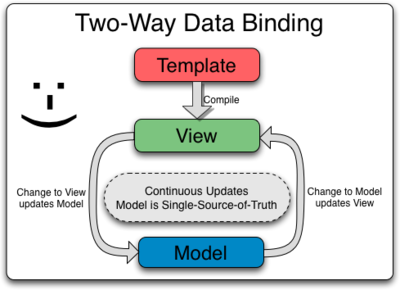
\includegraphics[width=0.5\textwidth]{res/Two_Way_Data_Binding}
	\caption{AngularJS two-way data binding: \url{https://docs.angularjs.org/guide/databinding}}
	\label{fig:tw-databinding}
\end{figure}


\subsection{Dependency Injection (DI)}
Dependency injection (DI) is a specialization of the \textit{inversion of control} pattern and has been named by \cite{fowler2004inversion}. \\
AngularJS adds DI to JavaScript, which allows the integration of dependencies into a specific controller, without making it globally available in the application. This ensures the availability of a component to specific controllers only.\\
It is hereby possible to use existing components and create own modules that can be used anywhere throughout the application. This allows decoupling of components, prevents the necessity for duplicate code and makes it easy to pull in 3rd party dependencies. 


\subsection{Angular Example}
The following example takes advantage of the concepts mentioned in the sections above. \\
Line 2 of listing \ref{lst:angular} defines the \textit{Fruits} factory. It returns a get get function, returning an array of fruits. In line 10, the \textit{FruitCtrl} controller is initiated. It uses dependency injection to take advantage of the Fruits factory. In line 11 the viewModel that is used to communicate with the view, is initiated. The following line adds a \textit{fruits} variable to the viewModel and calls the get function on the injected Fruits.\\
The view in listing \ref{lst:angular-view} specifies the angular app and the controller in line 1. In line 3, the \textit{ng-repeat} directive is used to iterate over the fruits from the viewModel. Listing \ref{lst:angular-result} shows the result.

\begin{lstlisting}[language=javascript, caption=AngularJS directive and controller definition, label=lst:angular]
angular.module("myApp", [])
  .factory('Fruits', function() {
    return {
      get: function() {
        return ["apple", "orange", "raspberry"];
      }
    };
  })
  
  .controller("FruitCtrl", function(Fruits) { // inject Fruits
    var vm = this; // ViewModel
    vm.fruits = Fruits.get(); // call directive
  });
\end{lstlisting}

\begin{lstlisting}[language=html, caption=AngularJS template, label=lst:angular-view]
<div ng-app="myApp" ng-controller="FruitController as fruitCtrl">
  <ul>
    <li ng-repeat="fruit in fruitCtrl.fruits">
      {{fruit}}
    </li>
  </ul>
</div>
\end{lstlisting}

\begin{lstlisting}[language=html, caption=HTML result, label=lst:angular-result]
<ul>
  <li>apple</li>
  <li>orange</li>
  <li>raspberry</li>
</ul>
\end{lstlisting}
